 \documentclass[xcolor=dvipsnames,table]{beamer}
%o
%e

\usepackage{latexsym}
\usepackage [ansinew]{inputenc}
\usepackage[brazil]{babel}
\usepackage{amssymb} %Este e o AMS paquete
\usepackage{amsmath}
\usepackage{stmaryrd}
\usepackage{fancybox}
\usepackage{datetime}
\usepackage{enumitem}

\usepackage[T1]{fontenc}

%\usepackage{beamerthemesplit}
\usepackage{graphicx}
\usepackage{graphics}
\usepackage{url}
\usepackage{algorithmic}
\usepackage{algorithm}
\usepackage{acronym}
\usepackage{array}
\usepackage{colortbl}

\newtheorem{definicao}{Definio}
\newcommand{\tab}{\hspace*{2em}}

\usepackage{pifont}

\mode<presentation>
{
  %\definecolor{colortexto}{RGB}{153,100,0}
  \definecolor{colortexto}{RGB}{0,0,0}
  
% \setbeamersize{sidebar width left=0.5cm}
  \setbeamertemplate{background canvas}[vertical shading][ bottom=white!10,top=white!10]
%   \setbeamercolor{title}{fg=colortitulo!80!black,bg=blue!20!white}
%   \setbeamercolor{title}{bg=colortitulo!20!black}
%   \setbeamercolor{background canvas}{bg=colortitulo}
%   \setbeamercolor{frametitle}{fg=red}

  \setbeamercolor{normal text}{fg=colortexto} 

  \usetheme{Warsaw}
  %\logo{\includegraphics[width=2cm]{Images/ratonfuerte.jpg}}


%   \usefonttheme[onlysmall]{structurebold}
%   \usecolortheme{seahorse}
%  \usecolortheme[named={YellowOrange}]{structure}
%   \usecolortheme[named={Blue}]{structure}
%   \usecolortheme{crane}
%   \useoutertheme{default}
}
\setbeamertemplate{caption}[numbered]

\title{Constru��o de Tabelas-Verdade} 

\author{
  Esdras Lins Bispo Jr. \\ \url{esdraspiano@gmail.com}
  } 
 \institute{
  L�gica para Ci�ncia da Computa��o \\Bacharelado em Ci�ncia da Computa��o}
\date{\textbf{27 de mar�o de 2019} }

\logo{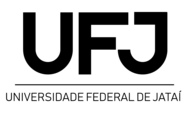
\includegraphics[width=1cm]{images/ufjJataiLogo.png}}

\begin{document}

	\begin{frame}
		\titlepage
	\end{frame}

	\begin{frame}{Plano de Aula}
		\tableofcontents
		%\tableofcontents[hideallsubsections]
	\end{frame}
	
	\section{Constru��o de Tabelas-Verdade}
	\begin{frame}{Constru��o de Tabelas-Verdade}
		\begin{block}{Exemplo 1}
			$P(p,q) =$ $\sim (p$ $\wedge \sim q)$
		\end{block} \pause
		\begin{block}{1� Resolu��o}
			\begin{center}
				\begin{tabular}{|cc|c|c|c|}
					\hline
					\onslide<3->{$p$}		&	\onslide<3->{$q$}	&	
					\onslide<8->{$\sim q$}	&	\onslide<10->{$p$ $\wedge \sim q$} &	\onslide<12->{$\sim (p$ $\wedge \sim q)$}	\\
					
					\hline
					
					\onslide<4->{V}	&	\onslide<6->{V}	&	\onslide<9->{F}	&	
					\onslide<11->{F}	&	\onslide<13->{V}	\\
					
					\onslide<4->{V}	&	\onslide<6->{F}	&	\onslide<9->{V}	&	
					\onslide<11->{V}	&	\onslide<13->{F}	\\
					
					\onslide<5->{F}	&	\onslide<7->{V}	&	\onslide<9->{F}	&	
					\onslide<11->{F}	&	\onslide<13->{V}	\\
					
					\onslide<5->{F}	&	\onslide<7->{F}	&	\onslide<9->{V}	&	
					\onslide<11->{F}	&	\onslide<13->{V}	\\
					\hline
				\end{tabular}
			\end{center}
		\end{block}
	\end{frame}

	\begin{frame}{Constru��o de Tabelas-Verdade}
		\begin{block}{Exemplo 1}
			$P(p,q) =$ $\sim (p$ $\wedge \sim q)$
		\end{block} \pause
		\begin{block}{2� Resolu��o}
			\begin{center}
				\begin{tabular}{|cc|c|c|c|c|c|}
					\hline
					\onslide<3->{$p$}		&	\onslide<3->{$q$}	&	
					\onslide<8->{$\sim$}	&	\onslide<9->{$(p$} &	\onslide<10->{$\wedge$}	&	\onslide<11->{$\sim$}	&
					\onslide<12->{$q)$}\\
					
					\hline
					
					\onslide<4->{V}		&	\onslide<6->{V}	&	\onslide<17->{V}	&	
					\onslide<13->{V}	&	\onslide<16->{F}	&	\onslide<15->{F}	&
					\onslide<14->{V}	\\
					
					\onslide<4->{V}		&	\onslide<6->{F}	&	\onslide<17->{F}	&	
					\onslide<13->{V}	&	\onslide<16->{V}	&	\onslide<15->{V}	&
					\onslide<14->{F}	\\
					
					\onslide<5->{F}		&	\onslide<7->{V}	&	\onslide<17->{V}	&	
					\onslide<13->{F}	&	\onslide<16->{F}	&	\onslide<15->{F}	&
					\onslide<14->{V}	\\
					
					\onslide<5->{F}		&	\onslide<7->{F}	&	\onslide<17->{V}	&	
					\onslide<13->{F}	&	\onslide<16->{F}	&	\onslide<15->{V}	&
					\onslide<14->{F}	\\
					
					\hline
				\end{tabular}
			\end{center}
		\end{block}
	\end{frame}

	\begin{frame}{Constru��o de Tabelas-Verdade}
		\begin{block}{Exemplo 1}
			$P(p,q) =$ $\sim (p$ $\wedge \sim q)$
		\end{block} \pause
		\begin{block}{3� Resolu��o}
			\begin{center}
				\begin{tabular}{|c|c|c|c|c|}
					\hline
					\onslide<8->{$\sim$}	&	\onslide<9->{$(p$} &	\onslide<10->{$\wedge$}	&	\onslide<11->{$\sim$}	&
					\onslide<12->{$q)$}\\
					
					\hline
					
					\onslide<17->{V}	&	\onslide<13->{V}	&	\onslide<16->{F}	&	\onslide<15->{F}	&	\onslide<14->{V}	\\
					
					\onslide<17->{F}	&	\onslide<13->{V}	&	\onslide<16->{V}	&	\onslide<15->{V}	&	\onslide<14->{F}	\\
					
					\onslide<17->{V}	&	\onslide<13->{F}	&	\onslide<16->{F}	&	\onslide<15->{F}	&	\onslide<14->{V}	\\
					
					\onslide<17->{V}	&	\onslide<13->{F}	&	\onslide<16->{F}	&	\onslide<15->{V}	&	\onslide<14->{F}	\\
					
					\hline
				\end{tabular}
			\end{center}
		\end{block}
	\end{frame}

\begin{frame}{Constru��o de Tabelas-Verdade}
	\begin{block}{Exemplo 2}
		$P(p,q) =$ $\sim (p \wedge q)$ $\vee \sim (q \leftrightarrow p)$
	\end{block} \pause
	\begin{block}{Exemplo 3}
		$P(p,q,r) = p$ $\vee \sim r \rightarrow q$ $\wedge \sim r$
	\end{block} \pause
	\begin{block}{Exemplo 5}
		$P(p,q,r) = (p \rightarrow (\sim q \vee r))$ $\wedge \sim (q \vee (p \rightarrow \sim r))$
	\end{block} \pause
\end{frame}

\begin{frame}{Valor L�gico de F�rmulas Compostas}
	\begin{block}{Exemplo 1}
		$P(p,q) =$ $\sim (p \vee q)$ $\leftrightarrow$ $\sim p$ $\wedge \sim q$
	\end{block} \pause
	\begin{block}{V(p) = V e V(q) = F}
		\begin{itemize}
			\item $V(\sim (p \vee q)$ $\leftrightarrow$ $\sim p$ $\wedge \sim q)$	\pause
			\item = $\sim (V(p) \vee V(q))$ $\leftrightarrow$ $\sim V(p)$ $\wedge \sim V(q))$	\pause
			\item = $\sim$ (V $\vee$ F$)$ $\leftrightarrow$ $\sim$ V $\wedge \sim$ F \pause
			\item = $\sim$ (V) $\leftrightarrow$ F $\wedge$ V \pause
			\item = F $\leftrightarrow$ F \pause
			\item = V
		\end{itemize}
	\end{block}
\end{frame}

\begin{frame}{Uso de Par�ntesis}
	\begin{block}{Prop�sitos}
		\begin{itemize}[label=-]
			\item Evitar ambiguidades; e
			\item For�ar preced�ncia.
		\end{itemize}
	\end{block} \pause
	\begin{block}{Ordem de Preced�ncia}
		\begin{itemize}
			\item[(1)] $\sim$
			\item[(2)] $\wedge$ e $\vee$
			\item[(3)] $\rightarrow$
			\item[(4)] $\leftrightarrow$
		\end{itemize}
	\end{block} \pause
	\begin{block}{Quando houver a mesma preced�ncia...}
		Haver� associa��o a partir da esquerda.
	\end{block}
\end{frame}

	\begin{frame}
		\titlepage
	\end{frame}
	
\end{document}